\chapter{Introdução}
\section{Conceitos básicos}
Existem conceitos que permeiam todas as linguagens, tais como:
\begin{itemize}
    \item Constantes e Variáveis
    \item Palavras reservadas
    \item Expressões Aritméticas
    \item Expressões Lógicas
    \item Comandos de Atribuição
    \item Entrada/Saída de dados
\end{itemize}
Esta seção tem como objetivo situar o leitor sobre estes conceitos.
\subsection{Constantes e Variáveis}
Estes dois conceitos tem em comum a alocação de uma região de memória no computador para guardar dados, como pode ser visto na Figura \ref{fig:memSimples}, porém para as constantes esse dado não pode ser modificado após sua criação, já para variáveis pode-se mudá-lo quantas vezes forem necessárias. Em ambos os casos necessita-se também do tipo de dado a ser guardado pelo computador, isto varia de linguagem, porém os tipos padrões constiuem os seguintes:
\begin{figure}[!h]
    \centering
    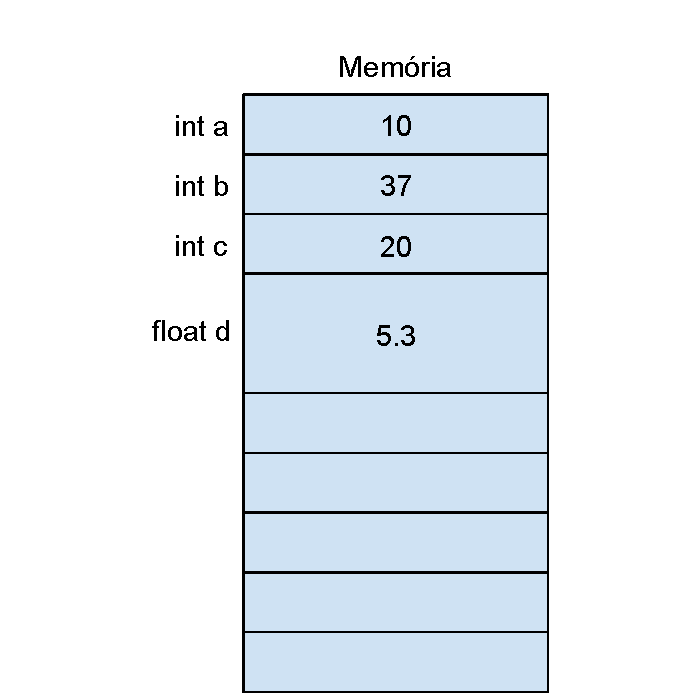
\includegraphics[scale=.5]{memSimples.pdf}
    \caption{Alocação de memória}
    \label{fig:memSimples}
\end{figure}
\begin{itemize}
    \item Númericos
    \begin{itemize}
        \item Inteiro - Ex.: 30, -15, 10, 0 ...
        \item Ponto Flutuante (Reais) - Ex.: 2.3, -1.2, 15.3 ...
    \end{itemize}
    \item Literais (Caracteres e Strings) - Ex.: "teste", "t", "sera" ...
    \item Lógicos (Booleano - Matemático George Boole) - Ex.: Verdadeiro e Falso
\end{itemize}
Em linguagens como C, C++ e Java há a necessidade de explicitar o tipo de dado ao se alocar a região de memória, em outras como Python ou PHP não há explicitamente o tipo ao se definir uma variável ou constante. \\
Exemplo em C e em seguida em Python:
\begin{lstlisting}
    //Comentario em C
    int a = 1;
    const int b = 2;
    float c = 2.3;
    const float d = 3.2;
    char e = 'a';
    const char f = 'b';
\end{lstlisting}
\begin{lstlisting}
    #Comentario em Python
    a = 1
    c = 2.3
    e = 'a'
\end{lstlisting}
Note que em Python não há a palavra const, não sendo possível criar constantes de verdade.
\subsection{Palavras reservadas}
Existem palavras reservadas que diferem de linguagem para linguagem, elas servem para diversas coisas, como definir um tipo de dado, declarar uma constante, dar comandos condicionais (se senão), comandos de repetição entre outros.
\subsection{Expressões Aritméticas}
Servem para fazer os cálculos utilizados no programa, os operadores mais comuns são: +, - , / , *.\\ 
Exemplo: $ a + b $
\subsection{Expressões Lógicas}
Fazer cálculos booleanos, que resultem em Verdadeiro ou Falso, os operadores mais comuns são: \&\& (E) e || (OU), existindo também os de maior que e menor que entre outros. E seus reultados seguem uma tabela verdade, como em \ref{tab:vE} e \ref{tab:vOU}.
Exemplo: \\
\begin{table}[!h]
\centering
\caption{Tabela verdade para operador E}
\label{tab:vE}
\begin{tabular}{llll} \hline \hline
0 & 1 &  &  \\
&   &  &  \\
&   &  &  \\ \hline \hline
\end{tabular}
\end{table}

\begin{table}[!h]
\centering
\caption{Tabela verdade para operador OU}
\label{tab:vOU}
\begin{tabular}{lll}
OU & F & V \\
F  & F & V \\
V  & V & V
\end{tabular}
\end{table}
\subsection{Comando de Atribuição}
Para atribuir um valor a uma variável tem-se o comando de atribuição, na maioria das linguagens se utiliza o comando '=' para tal. \\
Exemplo: $ a = 2 $ \\
Porém, algumas linguagens podem utilizar a sequência ``:='' entre outros.
\subsection{Entrada e Saída}
O computador esta configurado para ter uma saída padrão, o monitor, e uma entrada padrão, o teclado. Para acessar as estas funcionalidades, existem meios de requisitar a entrada de dados do usuário ou de mostrar algo na tela. Por didática será utilizado:
\begin{itemize}
    \item Print(<palavra>) - Para escrever na tela
    \item Input(<variavel>) - Para ler do teclado o que foi digitado
\end{itemize}
Mas vale lembrar que nas linguagens isto pode não estar desta forma, variando o comando para cada linguagem. Em C, por exemplo, o comando parar ler do teclado constitui o ``scanf()'' já para mostrar na tela o ``printf()''.

\section{Algoritmos}
Agora que sabemos alguns comandos de linguagens de programação podemos construir algoritmos simples, para tal devemos definir o que será o algoritmo: \\
\begin{definicao}{Algoritmo}
    Um algoritmo constitui uma sequência de passos finita, com instruções bem definidas e não ambíguas.
\end{definicao}
Vamos montar agora um problema para resolver a transformação de graus Celsius para Fahrenheit:
\begin{equation}
    T_{F} = T_{C} * \frac{9}{5} + 32
\end{equation}

\begin{lstlisting}
    real celsius, fahrenheit;
    Input(celsius)
    fahrenheit = celsius * (9/5) + 32
    Escreva(fahrenheit)
\end{lstlisting}